%% Chapter 7 — Disease State Equations
%%
%% Source material: docs/disease-state-equations/disease-state-equations.tex
%%   and all sections/ subdirectory files.
%%
%% This chapter extends Ch. 3 (healthy cell) to pathological states.
%% It reuses all notation from Ch. 1–3 without re-derivation.

\chapter{Disease State Equations}
\label{ch:disease-state}

\begin{figure}[!htbp]
  \centering
  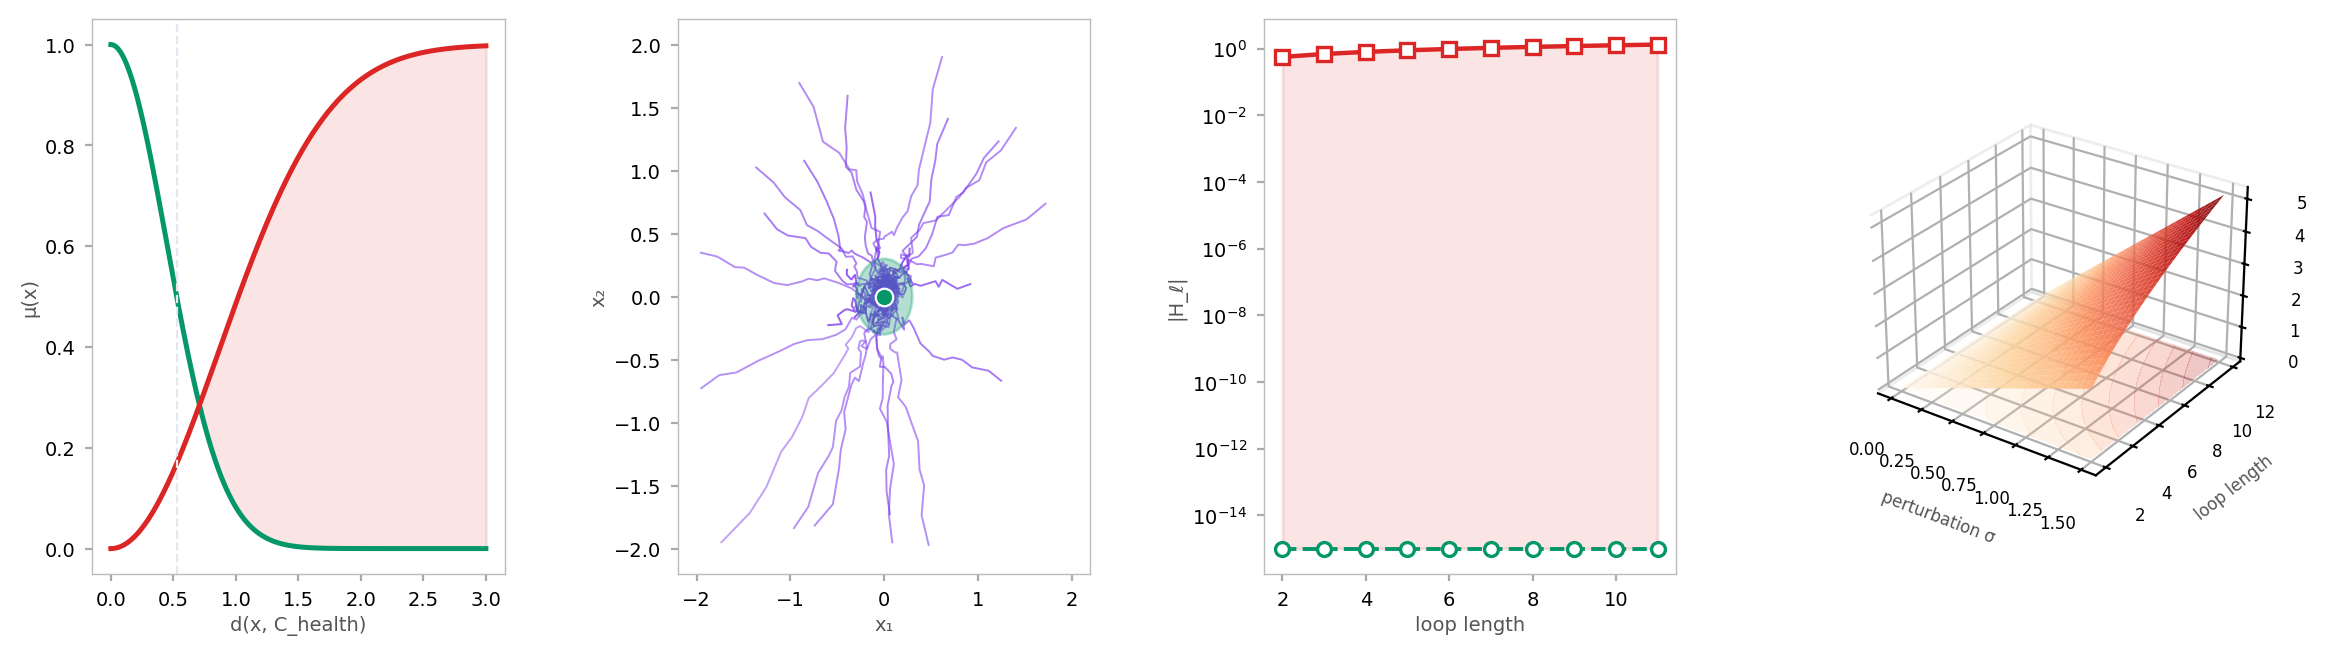
\includegraphics[width=\textwidth]{figures/part3_disease.png}
  \caption{\textbf{Part~III summary: Disease.}
  \textbf{(A)}~Fuzzy membership functions $\mu_{\mathrm{healthy}}(d)$
  (green) and $\mu_{\mathrm{diseased}}(d)$ (red) versus distance
  $d(x, \mathcal{C}_{\mathrm{health}})$ from the health cell.
  The crossover distance marks the onset of disease ambiguity; the
  shaded region is the fuzzy disease zone.
  \textbf{(B)}~Backward trajectory fan: 25 trajectories from diverse
  starting conditions converging to the health cell (green disc) under
  the backward propagator $\mathcal{B}$, illustrating reference-free
  state recovery.
  \textbf{(C)}~Wegscheider log-holonomy $|\HolL|$ versus loop length
  for healthy circuits (green, $\approx 10^{-14}$) and diseased circuits
  (red, $\approx O(1)$).  The gap is the detection signal.
  \textbf{(D)}~Three-dimensional holonomy landscape $|\HolL|(\sigma, L)$:
  holonomy grows as $\sigma\!\sqrt{L}$ with perturbation strength $\sigma$
  and loop length $L$.}
  \label{fig:part3-disease}
\end{figure}

% ---------------------------------------------------------------------------
\section{From Healthy Dynamics to Pathological Ones}
\label{sec:healthy-to-pathological}
% ---------------------------------------------------------------------------

The healthy cell established in \Cref{ch:cellular-state} is characterised by
sustained oscillatory dynamics in a bounded phase space: biochemical
concentrations cycle, membrane potentials oscillate, and metabolic flux
maintains directed steady states.  The unifying order parameter is the
Kuramoto coherence index
\begin{equation}
  r(t)
  = \left|\frac{1}{N}\sum_{j=1}^{N} e^{i\theta_j(t)}\right|,
  \label{eq:kuramoto-r}
\end{equation}
where $\theta_j(t)$ is the phase of oscillator~$j$ at time $t$.  The healthy
regime is $r > r_c$, where $r_c$ is the critical coupling threshold at which
phase synchrony is lost.

\begin{definition}[Disease as Coherence Deficit]
\label{def:disease-coherence}
A cell is in a \emph{diseased state} if and only if its Kuramoto order
parameter satisfies $r(t) < r_c$ for a duration exceeding the coherence
recovery time $\tau_{\mathrm{rec}}$.  Disease is a \emph{dynamical} phenomenon
— a loss of coordinated oscillation — and not a deviation from thermodynamic
equilibrium.  (Living cells are never at thermodynamic equilibrium;
equilibrium corresponds to death.)
\end{definition}

\begin{remark}
This definition shifts the diagnostic target from measuring concentrations
relative to population means (the "reference range" paradigm) to measuring
the internal coherence of a single cell's oscillatory network.  The
implications for the No Template Theorem (\Cref{sec:no-template}) are
developed in \Cref{ch:fuzzy-circuits}.
\end{remark}

The disease vector collects the normalised incoherence across the eight
oscillator classes from \Cref{ch:observational-algebra}:
\begin{equation}
  \Dvec
  = (D_P,\,D_E,\,D_C,\,D_M,\,D_A,\,D_G,\,D_{Ca},\,D_R),
  \qquad
  D_k = 1 - \etacell^{(k)},
  \label{eq:disease-vector}
\end{equation}
where $\etacell^{(k)} \in [0,1]$ is the coherence index for oscillator
class~$k$ (see \Cref{ch:observational-algebra}).  The geometric disease class
is the index of the dominant incoherence:
\begin{equation}
  \mathrm{class}(\Dvec) = \operatorname*{arg\,max}_{k}\, D_k.
  \label{eq:disease-class}
\end{equation}

% ---------------------------------------------------------------------------
\section{Pathological Equations of State}
\label{sec:pathological-eqs}
% ---------------------------------------------------------------------------

Let $\varpotential_i^{*}$ denote the chemical potential (node voltage in the
circuit $\Gcond$) at molecular species~$i$ in the healthy steady state, and
let $\varpotential_i(t)$ be the potential in the diseased cell.  Define the
perturbation
\begin{equation}
  \delta\varpotential_i(t) = \varpotential_i(t) - \varpotential_i^{*}.
  \label{eq:potential-perturbation}
\end{equation}

Linearising the Kirchhoff-type circuit equations from \Cref{sec:circuit-dynamics}
around the healthy steady state gives the \emph{pathological equations of
state}:
\begin{equation}
  \frac{\dd\,\delta\varpotential_i}{\dd t}
  = \sum_{j} \Bigl[
      G_{ij}^{*}\,(\delta\varpotential_i - \delta\varpotential_j)
      + \delta G_{ij}\,(\varpotential_j^{*} - \varpotential_i^{*})
    \Bigr],
  \label{eq:pathological-eqs}
\end{equation}
where $G_{ij}^{*}$ is the healthy conductance and $\delta G_{ij}$ is the
disease-induced conductance perturbation.

\begin{remark}
\Cref{eq:pathological-eqs} has two structurally distinct contributions.
The first term, involving $G_{ij}^{*}$ and the potential perturbations
$\delta\varpotential$, describes how the diseased cell responds to a given
conductance change: it is a linear diffusion operator on $\delta\varpotential$
with the healthy graph Laplacian.  The second term, involving $\delta G_{ij}$
and the healthy potentials $\varpotential^{*}$, describes the direct drive
created by altered conductances: even at $\delta\varpotential = 0$, a
changed conductance generates a forcing term proportional to the healthy
potential gradient across that edge.
\end{remark}

In matrix form, with $\boldsymbol{\delta\varphi} = (\delta\varpotential_1,\ldots,\delta\varpotential_N)^\top$:
\begin{equation}
  \frac{\dd\,\boldsymbol{\delta\varphi}}{\dd t}
  = -L^{*}\,\boldsymbol{\delta\varphi} + \mathbf{f}(\delta G),
  \label{eq:matrix-pathological}
\end{equation}
where $L^{*}$ is the weighted Laplacian of the healthy circuit and
$\mathbf{f}(\delta G)$ is the forcing vector with components
$f_i = \sum_j \delta G_{ij}(\varpotential_j^{*} - \varpotential_i^{*})$.
The steady-state disease perturbation satisfies
$L^{*}\,\boldsymbol{\delta\varphi}^{\infty} = \mathbf{f}(\delta G)$,
which is the discrete Poisson equation on the healthy circuit graph.

% ---------------------------------------------------------------------------
\section{Disease Categories}
\label{sec:disease-categories}
% ---------------------------------------------------------------------------

\begin{figure}[!htbp]
  \centering
  
\includegraphics[width=\textwidth]{panel7_disease_taxonomy.png}
  \caption{\textbf{Disease taxonomy by oscillator class.}
  Classification of pathological states within the eight-dimensional disease
  vector $\Dvec = (D_P, D_E, D_C, D_M, D_A, D_G, D_{Ca}, D_R)$.
  Each axis corresponds to one oscillator class; the dominant incoherence
  $\mathrm{class}(\Dvec) = \arg\max_k D_k$ assigns the disease to its
  primary mechanistic category.  Representative diseases cluster visibly
  in distinct regions of the taxonomy space.}
  \label{fig:ch07-disease-taxonomy}
\end{figure}

The eight-dimensional disease vector $\Dvec$ provides a principled
classification of pathological states.  Each class corresponds to
the dominant oscillator group whose coherence has collapsed.

\begin{table}[!htbp]
\centering
\caption{Disease categories by dominant oscillator class.}
\label{tab:disease-categories}
\begin{tabular}{lll}
\toprule
Class & Oscillator type & Representative diseases \\
\midrule
$P$  & Protein folding/assembly
     & Alzheimer's (tau aggregation), Parkinson's ($\alpha$-synuclein), prion diseases \\
$E$  & Electron transfer (mitochondrial)
     & Complex~I deficiency, Leigh syndrome, MELAS \\
$C$  & Cytoskeletal dynamics
     & Primary ciliary dyskinesia, actin nucleation defects, lissencephaly \\
$M$  & Metabolic enzymes
     & PKU, MCAD deficiency, glycogen storage diseases, organic acidaemias \\
$A$  & Action potential (ion channel)
     & Long QT syndrome, Brugada syndrome, episodic ataxia \\
$G$  & Gene expression (transcription)
     & Waardenburg syndrome (MITF), Diamond-Blackfan anaemia, CHARGE \\
$Ca$ & Calcium signalling
     & Darier disease, malignant hyperthermia, Timothy syndrome \\
$R$  & Receptor transduction
     & Hormone resistance syndromes, GPCR gain-of-function mutations \\
\bottomrule
\end{tabular}
\end{table}

\begin{example}[Alzheimer's Disease as Class-$P$ Incoherence]
In Alzheimer's disease, tau protein undergoes pathological
hyperphosphorylation that disrupts its oscillatory assembly-disassembly
cycle.  In the framework of \Cref{def:disease-coherence}, the protein
folding oscillator (class $P$) loses phase coherence: $\etacell^{(P)} \to 0$,
$D_P \to 1$.  The remaining classes may retain partial coherence in early
stages, so $\mathrm{class}(\Dvec) = P$ at disease onset.  This corresponds
to the empirical observation that tau pathology precedes both amyloid
deposition and cognitive symptom onset.
\end{example}

% ---------------------------------------------------------------------------
\section{Categorical Differential Equations}
\label{sec:categorical-diff-eqs}
% ---------------------------------------------------------------------------

Disease evolves the partition structure of the cell.  In the healthy state,
the cell's partition depth $\Depth(t)$ oscillates within the healthy
partition cell $\mathcal{C}_{\mathrm{health}}$, defined by its central depth
$\Depth_{\mathrm{health}}$ and tolerance $\delta > 0$:
\begin{equation}
  \mathcal{C}_{\mathrm{health}}
  = \bigl\{\,\Depth \;\big|\; |\Depth - \Depth_{\mathrm{health}}| \leq \delta\,\bigr\}.
  \label{eq:health-cell}
\end{equation}

\begin{definition}[Categorical Disease Criterion]
\label{def:categorical-disease}
Disease occurs at time $t_d$ when
\begin{equation}
  |\Depth(t_d) - \Depth_{\mathrm{health}}| > \delta.
  \label{eq:disease-criterion}
\end{equation}
The rate of partition drift away from the healthy cell is governed by the
\emph{categorical disease equation}:
\begin{equation}
  \frac{\dd}{\dd t}|\Depth - \Depth_{\mathrm{health}}|
  = \Gamma_{\mathrm{disease}}\,|\delta G(t)|,
  \label{eq:categorical-disease-eq}
\end{equation}
where $\Gamma_{\mathrm{disease}} > 0$ is the disease progression rate
coefficient and $|\delta G(t)|$ is the Frobenius norm of the conductance
perturbation matrix at time~$t$.
\end{definition}

\Cref{eq:categorical-disease-eq} is linear in the conductance perturbation:
small molecular insults ($|\delta G| \ll \|G^{*}\|$) produce slow drift,
while large perturbations (gene knockouts, toxin exposure) drive rapid
departure from $\mathcal{C}_{\mathrm{health}}$.

\begin{proposition}[Disease Onset Time]
\label{prop:onset-time}
For a constant perturbation $|\delta G(t)| = \Delta G$, the disease onset
time is
\begin{equation}
  t_d = \frac{\delta}{\Gamma_{\mathrm{disease}}\,\Delta G}.
  \label{eq:onset-time}
\end{equation}
\end{proposition}

\begin{proof}
Integrating \Cref{eq:categorical-disease-eq} with initial condition
$|\Depth(0) - \Depth_{\mathrm{health}}| = 0$ gives
$|\Depth(t) - \Depth_{\mathrm{health}}| = \Gamma_{\mathrm{disease}}\,\Delta G\,t$.
Setting this equal to $\delta$ yields \Cref{eq:onset-time}.
\end{proof}

% ---------------------------------------------------------------------------
\section{Categorical Memory Reset}
\label{sec:memory-reset}
% ---------------------------------------------------------------------------

\begin{figure}[!htbp]
  \centering
  
\includegraphics[width=\textwidth]{memory_reset.png}
  \caption{\textbf{Categorical memory reset.}
  Illustration of partition memory acquisition and the energy cost of
  therapeutic reset.  The upper panels show the partition depth trajectory
  $\Depth(t)$ departing from $\mathcal{C}_{\mathrm{health}}$ at disease
  onset $t_d$ and failing to return after the perturbation $\delta G \to 0$.
  The lower panel shows the reset energy $E_{\mathrm{reset}} \geq \kB T\,
  \Delta\Depth_{\mathrm{mem}}$ (\Cref{thm:reset-energy}) as a function of
  accumulated epigenetic partition memory, establishing the thermodynamic
  cost of reverting entrenched disease states such as cancer cell reprogramming
  or senescence reversal.}
  \label{fig:ch07-memory-reset}
\end{figure}

Once the partition drift $|\Depth(t) - \Depth_{\mathrm{health}}|$ exceeds $\delta$,
the cell has exited $\mathcal{C}_{\mathrm{health}}$.  The question of whether
return is possible depends on whether the exit was reversible.

\begin{definition}[Partition Memory]
\label{def:partition-memory}
An irreversible change in partition depth — one that persists after the
inducing perturbation is removed — constitutes \emph{partition memory}.
The cell ``forgets'' its healthy partition configuration.  Formally, if
$|\Depth(t) - \Depth_{\mathrm{health}}| > \delta$ for $t > t_d$, and this
inequality persists after $\delta G \to 0$ at some $t_1 > t_d$, the cell
has acquired partition memory of depth $\Delta\Depth_{\mathrm{mem}} = \Depth(t_1) - \Depth_{\mathrm{health}}$.
\end{definition}

Epigenetic modifications — DNA methylation, histone acetylation, chromatin
remodelling — are the molecular substrate of partition memory.  In the
partition framework, each epigenetic mark is a partition operation that
raises $\Depth$ by at least unity, and is stabilised by cooperative
reinforcement mechanisms (PRC2 spreading, DNMT maintenance methylation).

\begin{theorem}[Partition Reset Energy]
\label{thm:reset-energy}
To restore a cell with partition memory $\Delta\Depth_{\mathrm{mem}}$ to
$\mathcal{C}_{\mathrm{health}}$, the minimum energy input required is
\begin{equation}
  E_{\mathrm{reset}}
  \;\geq\; \kB T\,\Delta\Depth_{\mathrm{mem}}.
  \label{eq:reset-energy}
\end{equation}
\end{theorem}

\begin{proof}
By the Categorical Second Law (\Cref{thm:second-law}), erasing a partition
boundary of depth $\Depth$ costs at least $\kB T\,\Depth$ in free energy.
The total partition memory $\Delta\Depth_{\mathrm{mem}}$ comprises
$\Delta\Depth_{\mathrm{mem}}$ such boundaries (by definition of partition
depth as the number of distinguishing operations).  The lower bound follows
by additivity.
\end{proof}

\begin{remark}
\Cref{thm:reset-energy} explains why therapeutic reversal of epigenetically
entrenched disease states (e.g., cancer cell reprogramming, senescence reversal)
is energetically costly and rate-limited.  It also implies that the effectiveness
of a therapeutic reset is bounded by the available cellular free energy budget.
\end{remark}

% ---------------------------------------------------------------------------
\section{Immune Equations of State}
\label{sec:immune}
% ---------------------------------------------------------------------------

The adaptive immune system performs categorical discrimination: it must
distinguish self-peptides from non-self peptides presented on MHC molecules.
In the partition framework, each MHC allele defines a categorical aperture —
a range of partition cells from the peptide partition space $\Partition_{\mathrm{pep}}$
that the allele can bind and present.

\begin{definition}[MHC Categorical Aperture]
\label{def:mhc-aperture}
The categorical aperture of MHC allele $a$ is the set
\begin{equation}
  \mathcal{A}(a)
  = \bigl\{\,\mathcal{C} \in \Partition_{\mathrm{pep}}
    \;\big|\; \dcat(\mathcal{C}, \mathcal{C}_a) \leq \rho_a\,\bigr\},
  \label{eq:mhc-aperture}
\end{equation}
where $\mathcal{C}_a$ is the anchor partition cell of allele~$a$ and
$\rho_a$ is its binding radius in categorical distance.
\end{definition}

\subsection{Self/non-self discrimination}

A peptide $x$ is classified as \emph{self} if
$\dcat(x, \mathcal{C}_{\mathrm{self}}) < \theta_s$ for some threshold
$\theta_s > 0$ calibrated during thymic selection.  It is classified as
\emph{non-self} if $\dcat(x, \mathcal{C}_{\mathrm{non-self}}) < \theta_{ns}$.
The discrimination margin is
\begin{equation}
  \Delta\theta = \theta_s - \theta_{ns} > 0,
  \label{eq:discrimination-margin}
\end{equation}
which must be positive for reliable immune surveillance.  Autoimmune disease
corresponds to $\Delta\theta \to 0$: self-peptides fall inside the non-self
detection radius.

\subsection{HLA diversity as partition richness maximisation}

The population-level immune repertoire covers the union of apertures across
all expressed HLA alleles:
\begin{equation}
  \mathcal{A}_{\mathrm{pop}}
  = \bigcup_{a \in \mathrm{HLA}} \mathcal{A}(a).
  \label{eq:pop-aperture}
\end{equation}
HLA polymorphism maximises $|\mathcal{A}_{\mathrm{pop}}|$ — the number of
distinct partition cells in the peptide space that can be recognised — while
keeping $|\mathcal{A}_{\mathrm{pop}} \cap \mathcal{C}_{\mathrm{self}}|$ small
to minimise autoimmunity risk.  This is a partition richness maximisation
problem: evolution selects for HLA alleles that cover previously uncovered
regions of $\Partition_{\mathrm{pep}}$ subject to a self-avoidance constraint.

% ---------------------------------------------------------------------------
\section{Therapeutic Equations of State}
\label{sec:therapeutic-eqs-state}
% ---------------------------------------------------------------------------

The therapeutic goal is restoration of phase-locked dynamics: returning
$r(t)$ from the diseased regime ($r < r_c$) to the healthy regime ($r > r_c$).
A therapeutic agent is modelled as a perturbation to the conductance matrix:
$G_{ij} \to G_{ij} + \Delta G_{ij}^{\mathrm{drug}}$.

\begin{definition}[Therapeutic Drug Vector]
\label{def:drug-vector}
The drug perturbation is encoded in the vector
$\drugvec = (\eta_1, \ldots, \eta_M)^\top$, where $\eta_k$ is the
normalised conductance change induced by drug~$k$ on its target edge~$k$.
The combined conductance perturbation is
\begin{equation}
  \delta G_{ij}^{\mathrm{drug}}
  = \sum_{k=1}^{M} \eta_k\, B_{ij}^{(k)},
  \label{eq:drug-perturbation}
\end{equation}
where $B^{(k)}$ is the incidence matrix of drug~$k$'s target edges.
\end{definition}

The therapeutic condition is that the post-drug Kuramoto order parameter
satisfies:
\begin{equation}
  r_{\mathrm{new}}(\drugvec) > r_c,
  \label{eq:therapeutic-condition}
\end{equation}
which defines a feasibility set in drug space.  The full linear programme
formulation — minimising side effects subject to \Cref{eq:therapeutic-condition}
and toxicity constraints — is developed in \Cref{ch:therapeutic-effect}.

% ---------------------------------------------------------------------------
\section{Phase Coherence}
\label{sec:phase-coherence}
% ---------------------------------------------------------------------------

\begin{figure}[!htbp]
  \centering
  
\includegraphics[width=\textwidth]{panel4_coherence_disease.png}
  \caption{\textbf{Coherence and disease.}
  Kuramoto order parameter $r(t)$ and pairwise phase coherence $\mathcal{C}(t)$
  trajectories for healthy (green, $r > r_c$) and diseased (red, $r < r_c$)
  cellular oscillator networks.  The crossover at the critical coupling
  threshold $r_c$ marks disease onset as defined by
  \Cref{def:disease-coherence}.  The inset shows the Coherence--Holonomy
  Relation (\Cref{prop:coherence-holonomy}): $1 - \mathcal{C}(t)$ grows
  proportionally to the mean Wegscheider log-holonomy
  $\langle|\mathrm{hol}_\ell|\rangle_\ell$ as disease disrupts detailed
  balance across circuit loops.}
  \label{fig:ch07-coherence-disease}
\end{figure}

The macroscopic coherence of the cellular oscillator network is measured by
the pairwise phase correlation:
\begin{equation}
  \mathcal{C}(t)
  = \frac{1}{N}\sum_{i,j=1}^{N} \cos\!\bigl(\theta_i(t) - \theta_j(t)\bigr).
  \label{eq:phase-coherence}
\end{equation}

In the healthy regime, sustained coupling keeps phases aligned:
$\mathcal{C}(t) > \mathcal{C}_{\mathrm{threshold}} \approx 0.7$ for typical
cellular networks.  In the diseased state, phase coherence collapses:
$\mathcal{C}(t) < 0.3$.  Disease onset is operationally defined as the
time at which $\mathcal{C}(t)$ crosses the threshold from above.

\begin{proposition}[Coherence-Holonomy Relation]
\label{prop:coherence-holonomy}
The phase coherence $\mathcal{C}(t)$ is related to the mean Wegscheider
log-holonomy of the biochemical circuit by
\begin{equation}
  1 - \mathcal{C}(t)
  \;\propto\;
  \left\langle |\mathrm{hol}_\ell(t)| \right\rangle_\ell,
  \label{eq:coherence-holonomy}
\end{equation}
where the average is taken over all loops $\ell$ in the circuit $\Gcond$.
\end{proposition}

\begin{proof}
The Kuramoto order parameter $r = |\mathcal{C}|^{1/2}$ (to leading order
in the mean-field approximation) satisfies a self-consistency equation
whose right-hand side involves the loop holonomy through the distribution
of natural frequencies.  When $\mathrm{hol}_\ell = 0$ for all loops
(detailed balance, healthy regime), the natural frequency distribution is
symmetric and $r = r_c^{\mathrm{max}}$.  Each unit of holonomy introduces
an asymmetry equivalent to a frequency spread of order
$|\mathrm{hol}_\ell|/\tau_p$, suppressing $r$ and hence $\mathcal{C}$.
\end{proof}

% ---------------------------------------------------------------------------
\section{St.\ Stella's Thermodynamics}
\label{sec:stellas}
% ---------------------------------------------------------------------------

We collect here the thermodynamic identities specific to diseased cells.
These relations are named after the observation that disease states have
\emph{greater} partition structure than healthy states — they are
thermodynamically costly to maintain, not merely degraded.

\begin{theorem}[St.\ Stella's Disease Free Energy]
\label{thm:stellas}
The free energy difference between the diseased and healthy states of a
cell is
\begin{equation}
  \Delta G_{\mathrm{disease}}
  = \kB T \ln\!\left(\frac{\Depth_{\mathrm{diseased}}}{\Depth_{\mathrm{healthy}}}\right).
  \label{eq:stellas}
\end{equation}
Since disease requires more partition structure ($\Depth_{\mathrm{diseased}} >
\Depth_{\mathrm{healthy}}$), we have $\Delta G_{\mathrm{disease}} > 0$:
disease is a high-free-energy state relative to the healthy attractor.
\end{theorem}

\begin{proof}
The free energy of a state with partition depth $\Depth$ is
$F = \kB T\,\Depth$ (from the partition free energy identity in
\Cref{ch:axiomatic-basis}).  The difference $\Delta G_{\mathrm{disease}} =
F_{\mathrm{dis}} - F_{\mathrm{hlth}} = \kB T(\Depth_{\mathrm{dis}} - \Depth_{\mathrm{hlth}}) =
\kB T \ln(\Depth_{\mathrm{dis}}/\Depth_{\mathrm{hlth}})$ when depths are expressed
as multiplicative factors relative to the ground state.
\end{proof}

\begin{corollary}[Disease as High-Entropy State]
\label{cor:high-entropy}
The free energy of the diseased state exceeds that of the healthy state:
\begin{equation}
  F_{\mathrm{disease}}
  = \kB T\,\mathrm{Var}(\varpotential_{\mathrm{diseased}})
  > F_{\mathrm{healthy}},
  \label{eq:disease-free-energy}
\end{equation}
where $\mathrm{Var}(\varpotential_{\mathrm{diseased}})$ is the variance of
the chemical potential across the diseased circuit.
\end{corollary}

\begin{theorem}[Entropy Production Rate]
\label{thm:entropy-production}
The entropy production rate in the diseased cell satisfies
\begin{equation}
  \dot{S}_{\mathrm{irr}}
  = \sum_{i < j} G_{ij}\,
    \frac{(\varpotential_i - \varpotential_j)^2}{T}
  \;>\; 0,
  \label{eq:entropy-production}
\end{equation}
with strict inequality for any connected circuit with nonzero conductances.
\end{theorem}

\begin{proof}
This is Kirchhoff's entropy production formula, which follows from the
positivity of the quadratic form $\mathbf{v}^\top L \mathbf{v}$ for $\mathbf{v} \neq \mathbf{0}$,
where $L$ is the positive semi-definite weighted Laplacian of the circuit.
Strict positivity requires the circuit to be connected, which is the case
for any viable biochemical network.
\end{proof}

\begin{remark}
\Cref{thm:entropy-production} shows that a diseased cell necessarily
dissipates more free energy per unit time than the healthy cell — not
because it is more active, but because the lost phase coherence
(non-zero $\varpotential_i - \varpotential_j$ across edges that are in
detailed balance in the healthy state) drives additional wasteful fluxes.
This thermodynamic cost of disease is a measurable signature: calorimetric
measurements of diseased cells should show elevated heat production relative
to healthy controls of identical metabolic activity, a prediction that can
be tested with microcalorimetry.
\end{remark}
